%%%%%%%%%%%%%%%%%%%%%%%%%%%%%%%%%%%%%%%%%
% Programming/Coding Assignment
% LaTeX Template
%
% This template has been downloaded from:
% http://www.latextemplates.com
%
% Original author:
% Ted Pavlic (http://www.tedpavlic.com)
%
% Note:
% The \lipsum[#] commands throughout this template generate dummy text
% to fill the template out. These commands should all be removed when 
% writing assignment content.
%
% This template uses a Perl script as an example snippet of code, most other
% languages are also usable. Configure them in the "CODE INCLUSION 
% CONFIGURATION" section.
%
%%%%%%%%%%%%%%%%%%%%%%%%%%%%%%%%%%%%%%%%%

%----------------------------------------------------------------------------------------
%	PACKAGES AND OTHER DOCUMENT CONFIGURATIONS
%----------------------------------------------------------------------------------------

\documentclass{article}

\usepackage{fancyhdr} % Required for custom headers
\usepackage{lastpage} % Required to determine the last page for the footer
\usepackage{extramarks} % Required for headers and footers
\usepackage[usenames,dvipsnames]{color} % Required for custom colors
\usepackage{graphicx} % Required to insert images
\usepackage{subcaption}
\usepackage{listings} % Required for insertion of code
\usepackage{courier} % Required for the courier font
\usepackage{lipsum} % Used for inserting dummy 'Lorem ipsum' text into the template
\usepackage{amsfonts}
\usepackage{amssymb}
\usepackage{amsmath}
\usepackage{enumerate}
\usepackage{soul}
%Code for including Python code in Latex - outlined on the Piazza forum post, taken from Stackoverflow

\usepackage{enumitem}
\usepackage[utf8]{inputenc}
\definecolor{dkgreen}{rgb}{0,0.6,0}
\definecolor{gray}{rgb}{0.5,0.5,0.5}
\definecolor{mauve}{rgb}{0.58,0,0.82}

\lstset{frame=tb,
  language=Python,
  aboveskip=3mm,
  belowskip=3mm,
  showstringspaces=false,
  columns=flexible,
  basicstyle={\small\ttfamily},
  numbers=none,
  numberstyle=\tiny\color{gray},
  keywordstyle=\color{blue},
  commentstyle=\color{dkgreen},
  stringstyle=true{mauve},
  breaklines=true,
  breakatwhitespace=true,
  tabsize=3
}

% Margins
\topmargin=-0.45in
\evensidemargin=0in
\oddsidemargin=0in
\textwidth=6.5in
\textheight=9.0in
\headsep=0.25in

% Paragraph spacing
\setlength{\parskip}{10pt}


\linespread{1.1} % Line spacing

% Set up the header and footer
\pagestyle{fancy}
\lhead{\hmwkAuthorName} % Top left header
\chead{\hmwkClass\ (\hmwkClassTime): \hmwkTitle} % Top center head
%\rhead{\firstxmark} % Top right header
\lfoot{\lastxmark} % Bottom left footer
\cfoot{} % Bottom center footer
\rfoot{Page\ \thepage\ of\ \protect\pageref{LastPage}} % Bottom right footer

\setlength\parindent{0pt} % Removes all indentation from paragraphs

%----------------------------------------------------------------------------------------
%	CODE INCLUSION CONFIGURATION
%----------------------------------------------------------------------------------------

\definecolor{MyDarkGreen}{rgb}{0.0,0.4,0.0} % This is the color used for comments
\lstloadlanguages{Perl} % Load Perl syntax for listings, for a list of other languages supported see: ftp://ftp.tex.ac.uk/tex-archive/macros/latex/contrib/listings/listings.pdf
\lstset{language=Perl, % Use Perl in this example
        frame=single, % Single frame around code
        basicstyle=\small\ttfamily, % Use small true type font
        keywordstyle=[1]\color{Blue}\bf, % Perl functions bold and blue
        keywordstyle=[2]\color{Purple}, % Perl function arguments purple
        keywordstyle=[3]\color{Blue}\underbar, % Custom functions underlined and blue
        identifierstyle=, % Nothing special about identifiers                                         
        commentstyle=\usefont{T1}{pcr}{m}{sl}\color{MyDarkGreen}\small, % Comments small dark green courier font
        stringstyle=\color{Purple}, % Strings are purple
        showstringspaces=false, % Don't put marks in string spaces
        tabsize=5, % 5 spaces per tab
        %
        % Put standard Perl functions not included in the default language here
        morekeywords={rand},
        %
        % Put Perl function parameters here
        morekeywords=[2]{on, off, interp},
        %
        % Put user defined functions here
        morekeywords=[3]{test},
       	%
        morecomment=[l][\color{Blue}]{...}, % Line continuation (...) like blue comment
        numbers=left, % Line numbers on left
        firstnumber=1, % Line numbers start with line 1
        numberstyle=\tiny\color{Blue}, % Line numbers are blue and small
        stepnumber=5 % Line numbers go in steps of 5
}

% Creates a new command to include a perl script, the first parameter is the filename of the script (without .pl), the second parameter is the caption
\newcommand{\perlscript}[2]{
\begin{itemize}
\item[]\lstinputlisting[caption=#2,label=#1]{#1.pl}
\end{itemize}
}

%----------------------------------------------------------------------------------------
%	DOCUMENT STRUCTURE COMMANDS
%	Skip this unless you know what you're doing
%----------------------------------------------------------------------------------------

% Header and footer for when a page split occurs within a problem environment
\newcommand{\enterProblemHeader}[1]{
%\nobreak\extramarks{#1}{#1 continued on next page\ldots}\nobreak
%\nobreak\extramarks{#1 (continued)}{#1 continued on next page\ldots}\nobreak
}

% Header and footer for when a page split occurs between problem environments
\newcommand{\exitProblemHeader}[1]{
%\nobreak\extramarks{#1 (continued)}{#1 continued on next page\ldots}\nobreak
%\nobreak\extramarks{#1}{}\nobreak
}

\setcounter{secnumdepth}{0} % Removes default section numbers
\newcounter{homeworkProblemCounter} % Creates a counter to keep track of the number of problems
\setcounter{homeworkProblemCounter}{-1}

\newcommand{\homeworkProblemName}{}
\newenvironment{homeworkProblem}[1][Problem \arabic{homeworkProblemCounter}]{ % Makes a new environment called homeworkProblem which takes 1 argument (custom name) but the default is "Problem #"
\stepcounter{homeworkProblemCounter} % Increase counter for number of problems
\renewcommand{\homeworkProblemName}{#1} % Assign \homeworkProblemName the name of the problem
\section{\homeworkProblemName} % Make a section in the document with the custom problem count
\enterProblemHeader{\homeworkProblemName} % Header and footer within the environment
}{
\exitProblemHeader{\homeworkProblemName} % Header and footer after the environment
}

\newcommand{\problemAnswer}[1]{ % Defines the problem answer command with the content as the only argument
\noindent\framebox[\columnwidth][c]{\begin{minipage}{0.98\columnwidth}#1\end{minipage}} % Makes the box around the problem answer and puts the content inside
}

\newcommand{\homeworkSectionName}{}
\newenvironment{homeworkSection}[1]{ % New environment for sections within homework problems, takes 1 argument - the name of the section
\renewcommand{\homeworkSectionName}{#1} % Assign \homeworkSectionName to the name of the section from the environment argument
\subsection{\homeworkSectionName} % Make a subsection with the custom name of the subsection
\enterProblemHeader{\homeworkProblemName\ [\homeworkSectionName]} % Header and footer within the environment
}{
\enterProblemHeader{\homeworkProblemName} % Header and footer after the environment
}

%----------------------------------------------------------------------------------------
%	NAME AND CLASS SECTION
%----------------------------------------------------------------------------------------

\newcommand{\hmwkTitle}{Assignment 2 - Deep NN} % Assignment title
\newcommand{\hmwkDueDate}{Friday,\ February 23,\ 2018} % Due date
\newcommand{\hmwkClass}{CSC2515} % Course/class
\newcommand{\hmwkClassTime}{L0101} % Class/lecture time
\newcommand{\hmwkAuthorName}{M.Wong, S.Pyda} % Your name

%----------------------------------------------------------------------------------------
%	TITLE PAGE
%----------------------------------------------------------------------------------------

\title{
\vspace{2in}
\textmd{\textbf{\hmwkClass:\ \hmwkTitle}}\\
\normalsize\vspace{0.1in}\small{Due\ on\ \hmwkDueDate}\\
\vspace{0.1in}
\vspace{3in}
}

\author{\textbf{\hmwkAuthorName}}
%\date{} % Insert date here if you want it to appear below your name

%----------------------------------------------------------------------------------------

\begin{document}

\maketitle
\clearpage
%----------------------------------------------------------------------------------------
%	Introduction
%----------------------------------------------------------------------------------------

\begin{homeworkProblem}

\noindent \textit{Introductory information and readme instructions}

This submissions containts the required files:  \textit{digits.py, faces.py, deepfaces.py, deepnn.tex  \& faces.pdf} in addition to two folders - both containing an previously downloaded pictures for each actor/actress. The downloading code can be found in the source files.  Comments about the code are located in each of the source files. Code was written in Python 3.5 with the Anaconda environment - the packages used are outlined at the beginning of the file.



\end{homeworkProblem}
\clearpage
%----------------------------------------------------------------------------------------
%	PROBLEM 1
%----------------------------------------------------------------------------------------

% To have just one problem per page, simply put a \clearpage after each problem

\begin{homeworkProblem}

\noindent \textit{Dataset description}

In parts 1 through , the MNIST dataset of handwritten digits will be used: \textit{mnist\_all.mat}. The data is loaded in the form of a python dictionary. It is already split into training and testing sets - with 60 000 digits in the training and 10 000 in testing, and is also split by digit which can be accessed with \textit{train[digit]}. The number of of each digit in test/train is approximately equal although there are variations between digits. The digit data is in the form of a 784 integer array, representing the flattened pixel intensities of 28 by 28 pixel images. 
\\

10 examples of each digit are shown below:
\\

\begin{center}
\begin{figure}[!ht]\centering
\begin{subfigure}{.3\textwidth}\centering
  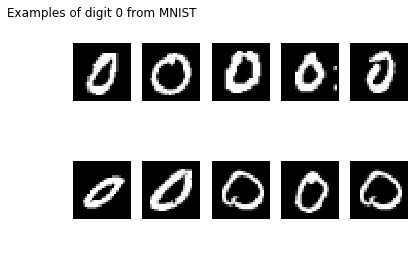
\includegraphics[scale=0.3]{Mnist0.jpg}
\end{subfigure}
\begin{subfigure}{.3\textwidth}\centering
  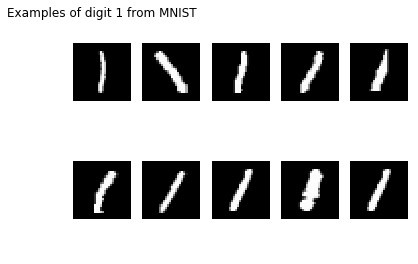
\includegraphics[scale=0.3]{Mnist1.jpg}
\end{subfigure}
\begin{subfigure}{.3\textwidth}\centering
  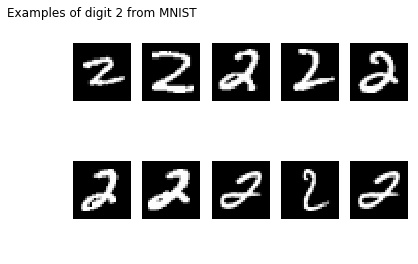
\includegraphics[scale=0.3]{Mnist2.jpg}
\end{subfigure}
\begin{subfigure}{.3\textwidth}\centering
  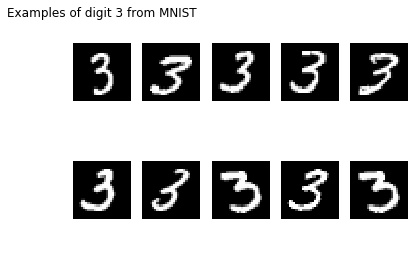
\includegraphics[scale=0.3]{Mnist3.jpg}
\end{subfigure}
\begin{subfigure}{.3\textwidth}\centering
  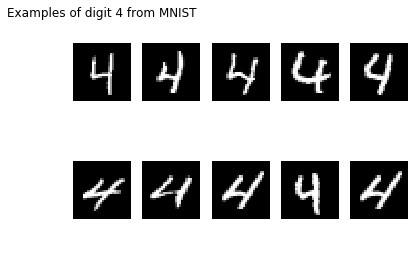
\includegraphics[scale=0.3]{Mnist4.jpg}
\end{subfigure}
\begin{subfigure}{.3\textwidth}\centering
  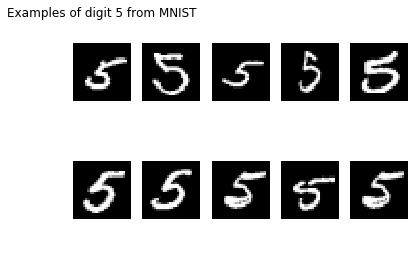
\includegraphics[scale=0.3]{Mnist5.jpg}
\end{subfigure}
\begin{subfigure}{.3\textwidth}\centering
  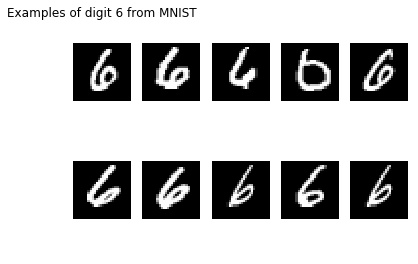
\includegraphics[scale=0.3]{Mnist6.jpg}
\end{subfigure}
\begin{subfigure}{.3\textwidth}\centering
  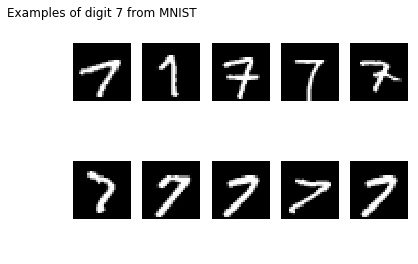
\includegraphics[scale=0.3]{Mnist7.jpg}
\end{subfigure}
\begin{subfigure}{.3\textwidth}\centering
  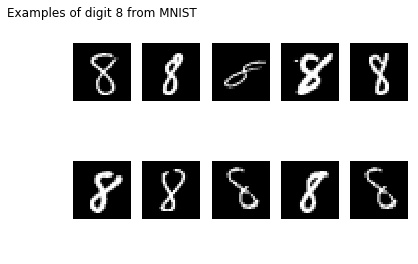
\includegraphics[scale=0.3]{Mnist8.jpg}
\end{subfigure}
\begin{subfigure}{.3\textwidth}\centering
  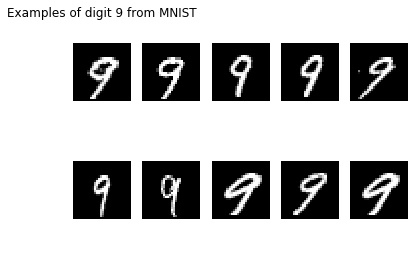
\includegraphics[scale=0.3]{Mnist9.jpg}
\end{subfigure}
\caption{Digits from MNIST}
\end{figure}
\end{center}



\end{homeworkProblem}
\clearpage
%----------------------------------------------------------------------------------------
%	PROBLEM 2
%----------------------------------------------------------------------------------------

\begin{homeworkProblem}
\noindent \textit{Computation of the provided Network.}
\\

The network provided in Part 2 is shown below:

  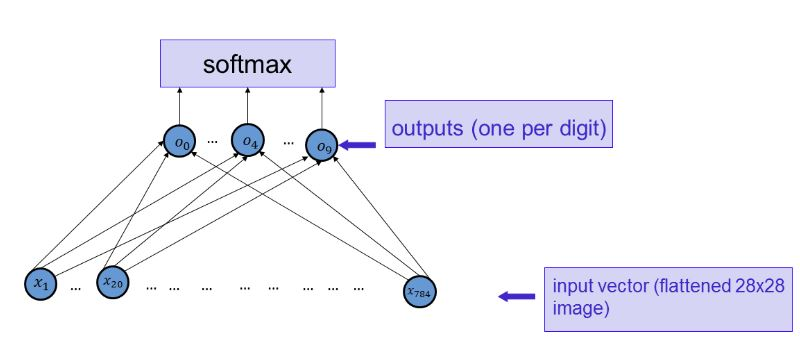
\includegraphics[scale=0.3]{Mnist-Question2.jpg}

The source code to compute the assigned network is provided below.
\begin{lstlisting}
def compute(X, W, b):
    hypothesis = np.matmul(W.T, X)
    hypothesis = hypothesis + b
    return hypothesis
\end{lstlisting}

The source code running a test case of the assigned network is provided below, followed by the output.  M is the MNIST dataset provided, W and b are randomly initialized numpy variables.
\begin{lstlisting}
def testPart2():
    # Load Data
    M = loadData()
    train = loadTrain(M)
    # Testing computation function
    # Initialize weights and bias to random normal variables
    W = np.random.normal(0.0, 0.1, (784, 10))
    b = np.random.normal(0, 0.1, (10, 1))
    hypothesis = compute(train, W, b)
    print(softmax(hypothesis))
\end{lstlisting}

Output (after applying softmax) from the test case:
\begin{lstlisting}
[[ 0.02681158  0.0532326   0.04155301 ...,  0.02401518  0.05461363
   0.09298066]
 [ 0.02934882  0.02945978  0.00866719 ...,  0.02812303  0.05160524
   0.06640991]
 [ 0.07800929  0.14095711  0.05324094 ...,  0.08344358  0.071218
   0.03403779]
 ..., 
 [ 0.06811845  0.09068319  0.11408343 ...,  0.09293973  0.23242635
   0.24750088]
 [ 0.42558937  0.28527524  0.36294473 ...,  0.32821263  0.12923604
   0.11150445]
 [ 0.04023265  0.03443131  0.05201543 ...,  0.0454216   0.06806685
   0.08509415]]
\end{lstlisting}
\end{homeworkProblem}
\clearpage


%----------------------------------------------------------------------------------------
%	PROBLEM 3
%----------------------------------------------------------------------------------------

\begin{homeworkProblem}
\noindent \textit{Gradient derivation and vectorized format}

\begin{enumerate}[label=(\Alph*)]
\item 

For the network described above, the cost function used will be the sum of negative log-probabilities.
\\
This cost function, summed over training examples is:
\\
$C=-\sum_jy_jlogp_j$
\\
Where y is the actual target and p is the predicted value.
\\
The output $p_i$ is the calculated the softmax function to $o_i$,:
\\
$p_i=\frac{e^{o_i}}{\sum_je^{o_j}}$, \hspace{0.25cm} $o_i=\sum_jx_jw_{ij}$
\\
We use the chain rule to find $\frac{dC}{dw_{ij}}$:
\\
$\frac{dC}{dw_{ij}}=\frac{dC}{dp_i}\frac{dp_i}{do_i}\frac{do_i}{dw_{ij}}$
\\
$\frac{dp_i}{do_i}=\frac{e^{o_i}}{\sum_je^{o_i}}-\big( \frac{e^{o_i}}{\sum_je^{o_i}}\big)^2=p_i(1-p_i)$
\\
$\frac{do_i}{dw_{ij}}=x_j$
\\
$\frac{dC}{do_i}=\sum_j\frac{dC}{dp_j}\frac{dp_j}{do_i}$



\item The source code for computing the gradient is shown below.
\begin{lstlisting}
def grad_NLL_W(y, o, layer):
    p = softmax(o)
    grad = p - y
    grad = np.matmul(grad, np.transpose(layer))
    return np.transpose(grad)


# Computes the gradient of negative log-loss function for biases only
def grad_NLL_b(y, o):
    p = softmax(o)
    grad = p - y
    grad = np.sum(grad, axis=1, keepdims=True)
    return grad
\end{lstlisting}
The source for our test cases, along with the outputs, are also shown below.
\begin{lstlisting}
def testPart3():
    # Test gradient functionality
    y = np.zeros((10, 1))
    y[1, :] = 1

    # Create a test matrix
    M = loadData()
    test0 = ((M["train1"][130].T) / 255.0).reshape((784, 1))
    W = np.random.normal(0, 0.2, (784, 10))
    b = np.random.normal(0, 0.2, (10, 1))
    # print(np.where(test0 != 0))

    # Create a finite difference
    h = 0.00001

    # Weight testing
    finite_W = np.zeros((784, 10))
    finite_W[542, 0] = h
    finite_d = (NLL(y, compute(test0, W + finite_W, b)) - NLL(y, compute(test0, W, b))) / (h)
    print("Cost for row 542, column 0: " + str(finite_d))
    gradient = grad_NLL_W(y, compute(test0, W, b), test0)
    print("Gradient for row 542, column 0: " + str(gradient[542, 0]))

    # Bias testing
    finite_b = np.zeros((10, 1))
    finite_b[1, :] = h
    finite_d = (NLL(y, compute(test0, W, b + finite_b)) - NLL(y, compute(test0, W, b))) / (h)
    print("Cost for second element in bias: " + str(finite_d))
    gradient = grad_NLL_b(y, compute(test0, W, b))
    print("Gradient matrix: " + str(gradient))

    # Reinitialize test variables for another test
    finite_W = np.zeros((784, 10))
    finite_b = np.zeros((10, 1))
    y = np.zeros((10, 1))
    test1 = ((M["train9"][130].T) / 255.0).reshape((784, 1))
    y[9, :] = 1

    # Weight testing
    finite_W[300, 4] = h
    finite_d = (NLL(y, compute(test1, W + finite_W, b)) - NLL(y, compute(test1, W, b))) / (h)
    print("Cost for row 300, column 4: " + str(finite_d))
    gradient = grad_NLL_W(y, compute(test1, W, b), test1)
    print("Gradient for row 300, column 4: " + str(gradient[300, 4]))

    # Bias testing
    finite_b[4, :] = h
    finite_d = (NLL(y, compute(test1, W, b + finite_b)) - NLL(y, compute(test1, W, b))) / (h)
    print("Cost for fifth element in bias: " + str(finite_d))
    gradient = grad_NLL_b(y, compute(test1, W, b))
    print("Gradient matrix: " + str(gradient))

\end{lstlisting}
\begin{lstlisting}
Cost for row 542, column 0: 0.0424078520744
Gradient for row 542, column 0: 0.0424076964593
Cost for second element in bias: -0.996437311773
Gradient matrix: [[ 0.05461597]
 [-0.99643733]
 [ 0.03592502]
 [ 0.32774037]
 [ 0.04444944]
 [ 0.05179153]
 [ 0.08930539]
 [ 0.14572631]
 [ 0.19441422]
 [ 0.05246907]]
Cost for row 300, column 4: 0.000106382902487
Gradient for row 300, column 4: 0.000106382357955
Cost for fifth element in bias: 0.00010680176743
Gradient matrix: [[  3.36017608e-03]
 [  1.57850465e-02]
 [  1.07051677e-02]
 [  1.06504072e-01]
 [  1.06801186e-04]
 [  6.75277789e-02]
 [  9.15366897e-02]
 [  8.16717644e-02]
 [  6.16811862e-01]
 [ -9.94009358e-01]]
\end{lstlisting}
\end{enumerate}


\end{homeworkProblem}
\clearpage
%----------------------------------------------------------------------------------------
%	PROBLEM 4
%----------------------------------------------------------------------------------------

\begin{homeworkProblem}
\noindent \textit{Gradient Descent Training}

For the Vanilla Gradient Descent algorithm, the weights and biases were sampled from the normal distribution around a mean of 0 and standard deviation of 0.2, using \textit{numpy.random.normal}. The weights and biases were initialized with shapes (784, 10) and (10, 1) respectively. 
\\

The optimization procedure for gradient descent involved testing: the type of distribution used in weight and bias initializiation, the learning rate, and the number of iterations. The reported results proved to be optimial.  The  network converges relatively quickly at 500 iterations - although itwas tested up to approximately 5000 iterations, however this had little accuracy on validation performance. The learning curve is shown below. 


By trial and error, a learning rate of 0.00001 was selected. The learning rate was chosen to optimize convergence time - a low learning rate resulted in slow convergence time, and a high learning rate resulted in fluctuations and hindered convergence.  
\\

The log loss is plotted against the number of iterations ( at this stage different methods are being compared for the same number of training examples so it was not necessary to divide loss by number of examples). 
\\

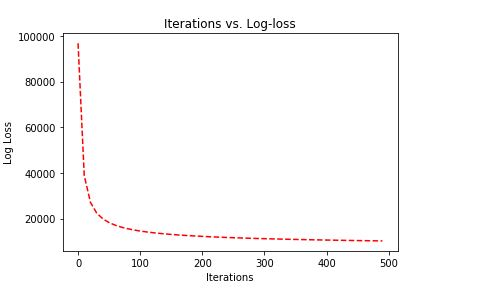
\includegraphics[scale=1]{Mnist-Question4.jpg}


\end{homeworkProblem}
\clearpage
%----------------------------------------------------------------------------------------
%----------------------------------------------------------------------------------------
%	PROBLEM 5
%----------------------------------------------------------------------------------------

\begin{homeworkProblem}
\noindent \textit{Gradient Descent With Momentum}
\\

Momentum is used in gradient descent to dampen oscillation and include an directional accumulation term to increase speed:
\\
The paramter update rule for momentum, as  provided in lecture notes is:
\\

$\nu\leftarrow\gamma\nu+\alpha\frac{dC}{dW}$
\\
$W\leftarrow W-\nu$
\\

Where $\gamma$ is the momentum term and $\alpha$ is the learning rate. C is the cost, and W is the parameter (weight) being updated. 
The momentum rate was set to 0.5 based on some initial tests, however the number could be optimized further for better/faster performance. This momentum rate was sufficient to demonstrate its effect.
\\
The function for vectorized momentum is shown below.

\begin{lstlisting}
\# MOMENTUM GRADIENT DESCENT
    
def grad_descent_w(NLL, grad_NLL_W, grad_NLL_b, x, y, init_w, init_b, alpha, iterations):
    iters = list()
    costy = list()

    EPS = 1e-5
    prev_w = init_w - 10 * EPS
    prev_b = init_b - 10 * EPS
    w = init_w.copy()
    b = init_b.copy()
    max_iter = iterations
    iter = 0

    v = np.zeros((784, 10))
    v[:, :] = 0.000001  # Initialize
    momentum_rate = 0.5

    while np.linalg.norm(w - prev_w) > EPS and iter < max_iter and np.linalg.norm(b - prev_b) > EPS:
        prev_w = w.copy()
        prev_b = b.copy()
        grad_desc = alpha * (grad_NLL_W(y, compute(x, w, b), x))
        mv = np.multiply(momentum_rate, v)
        v = np.add(mv, grad_desc)
        w -= v
        b -= alpha * (grad_NLL_b(y, compute(x, w, b)))
        if iter % 10 == 0:
            print("Iteration: " + str(iter))
            print("Cost: " + str(NLL(y, compute(x, w, b))))
            cost_i = NLL(y, compute(x, w, b))
            iters.append(iter)
            costy.append(cost_i)
        iter += 1
\end{lstlisting}

The figure below shows the learning curve on train data for gradient descent with and without momentum. It can be observed that momentum increases convergence speed.

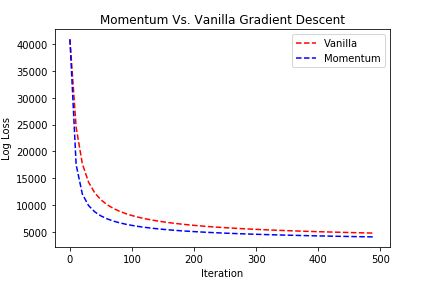
\includegraphics[scale=1]{Mnist-Question5.jpg}


\end{homeworkProblem}
\clearpage
%----------------------------------------------------------------------------------------
%----------------------------------------------------------------------------------------
%	PROBLEM 6
%----------------------------------------------------------------------------------------

\begin{homeworkProblem}
\noindent \textit{Contours of Gradient Descent}

In this section, the effectiveness of gradient descent moving towards a minima will be demonstrated on contour plots. The weights chosen were at $init\_w[490,3]$ and  $init\_w[490,3]$. These weights were chosen because by checking the corresponding values on the digits, to ensure that they were not all 0s would not have an effect on the output. When the weights were allowed to vary around the vales obtained in Part 5, without gradient descent, they did not move towards the local minima. 
\\
The weights were moved $\pm$ 0.15 from their trained values. The learning rate was increased to 0.017, and 20 iterations were run.
\\
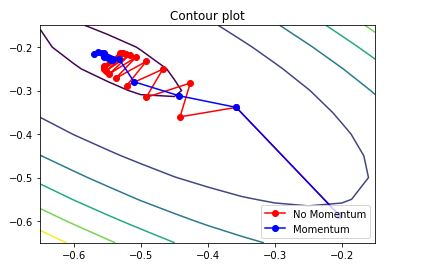
\includegraphics[scale=1]{Mnist-Question6.jpg}
\\
As shown in the figure momentum results in a faster path towards the minimum with fewer oscillations. The momentum term in the update introduces memory and allows the learning process to accelerate in consistent directions. 
\\

An example of momentum not being effective, would be as stated above, where the weights correspond to pixels of 0 or close to 0. In the example below, the weights chosen were changed to at $init\_w[10,3]$ and $init\_w[11,3]$, which may have been closer to the sides. It can be seen from the contours that they are more linear and  less effected by the weights. Momentum could be less effective, or very similar to vanilla gradient descent, when there is already a 'smooth' path towards the minima.

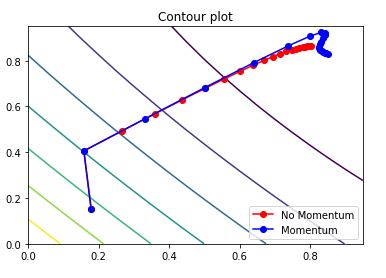
\includegraphics[scale=1]{Mnist-Question6e.jpg}

\end{homeworkProblem}
\clearpage
%----------------------------------------------------------------------------------------
%	PROBLEM 7
%----------------------------------------------------------------------------------------
\begin{homeworkProblem}

Running the linear regression classifier results in a training accuracy of $89\%$ and a validation accuracy of $56\%$.  Both the $\alpha$ and number of iterations were modified, to varying degrees of success - however, it is worth noting that the validation accuracy is significantly lower than the training accuracy which may be a symptom of overfitting.
\par Two loops were written in order to obtain the training hypothesis and validation hypothesis labels.  The steps are written below.
\begin{enumerate}
\item A matrix of 0's was initialized to the same shape as that of the label matrix
\item Each column in the label matrix was scanned for it's maximum value and the index of that value was stored in a new variable, \textit{max}
\item Starting at the $0^{th}$ column, a 1 was stored into the 0's matrix for each index in \textit{max}, and iterated through until the last column was reached.
\item The resultant matrix now had only one value of 1 in each column and was compared to the label matrix.
\end{enumerate}
An example of this for the training data is shown below.
\begin{lstlisting}
    #Training hypothesis
    ones_t = np.ones((1,training.shape[1]))
    training_with_bias = vstack((ones_t,training))
    training_hypothesis = np.matmul(theta.T,training_with_bias)
    max = training_hypothesis.argmax(axis=0)
    max = np.array(max)
    training_hypothesis_labels = np.zeros((training_hypothesis.shape))
    print(training_hypothesis_labels.shape)
    i = 0
    while i < training_hypothesis_labels.shape[1]:
        index = max[i]
        training_hypothesis_labels[index,i]=1
        i+=1

    correct = 0
    i = 0
    while i < training_hypothesis_labels.shape[1]:
        if np.array_equal(training_hypothesis_labels[:,i],training_labels[:,i]) is True:
            correct += 1
        i+=1
    print("Training accuracy is: " + str(correct/600.0))

\end{lstlisting}

\end{homeworkProblem}
\clearpage
%----------------------------------------------------------------------------------------
%	PROBLEM 8
%----------------------------------------------------------------------------------------
\begin{homeworkProblem}
\noindent \textit{Training a single-hidden-layer fully connected network}

The provided source was modified to train a single-hidden layer, fully-connected neural network to classify actors and actresses from Project 1, assuming the original list of actors and actresses were the following:
\begin{lstlisting}
act =['Lorraine Bracco', 'Peri Gilpin', 'Angie Harmon', 'Alec Baldwin', 'Bill Hader', 'Steve Carell']
\end{lstlisting}

The neural network architecture involved a fully connected layer (Linear), followed by ReLU activation (activation), followed by another fully connected layer (Linear) with input dimensions of 32*32*3 (e.g. 32 $\times$ 32 $\times$ 3 representing the pixel areas and colour channels), 20 hidden neurons, and finally a output layer consisting of 6 output units.  The Cross Entropy cost was minimized as the cost function.  Furthermore, experimentation involving the learning rate, $\alpha$, number of iterations, as well as batch size was conducted, leading to an optimal learning rate of 0.0001, 5000 iterations, and a batch size of approximately 200 (out of a total 450 training examples).  After training, the accuracy for the training set, validation set and test set were 87.3\%, 84.9\% and 79.2\% respectively.  A plot of the training \& validation accuracies throughout the training are shown below.
\begin{center}
\begin{figure}[!ht]\centering
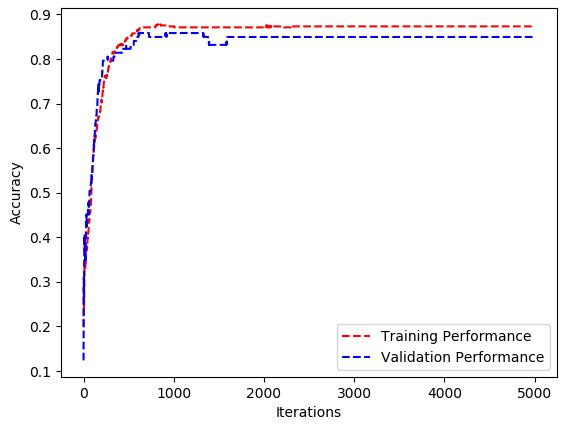
\includegraphics{Mnist-Question8.jpg}
\caption{Training \& Validation performance for Part 8}
\end{figure}

\end{center}

\end{homeworkProblem}
\clearpage

%----------------------------------------------------------------------------------------
%	PROBLEM 8
%----------------------------------------------------------------------------------------
\begin{homeworkProblem}
\noindent \textit{Visualizing $\theta 's$ with multiple label matrix}

The 6 figures below show the visualized $\theta 's$ for training on the full set of actors in $act$ with the label matrix, as outlined in the assignment specification.

A potential explanation for the lack of "face-like" appearance in $\theta 's $ obtained after training may be that the size of the training set is too large for each actor.  As observed in part 4, with only two actors from the Baldwin and Carell sets, the $\theta 's$ visualized more resembled faces.
\end{homeworkProblem}
\clearpage

%----------------------------------------------------------------------------------------
%	PROBLEM 8
%----------------------------------------------------------------------------------------
\begin{homeworkProblem}
\noindent \textit{Visualizing $\theta 's$ with multiple label matrix}

The 6 figures below show the visualized $\theta 's$ for training on the full set of actors in $act$ with the label matrix, as outlined in the assignment specification.

A potential explanation for the lack of "face-like" appearance in $\theta 's $ obtained after training may be that the size of the training set is too large for each actor.  As observed in part 4, with only two actors from the Baldwin and Carell sets, the $\theta 's$ visualized more resembled faces.
\end{homeworkProblem}
\clearpage
\end{document}